\section{Úvod}

%% Co je UML, jak a proč ho používat

%%%%%%%%%%%%%%%%%%%%%%%%%%%%%%%%%%%%%%%%%%%%%%%%%%%%%%%%%%%%%%%%%%%%%%%%
%% Slide

\begin{frame}{Úvod}

\begin{figure}
	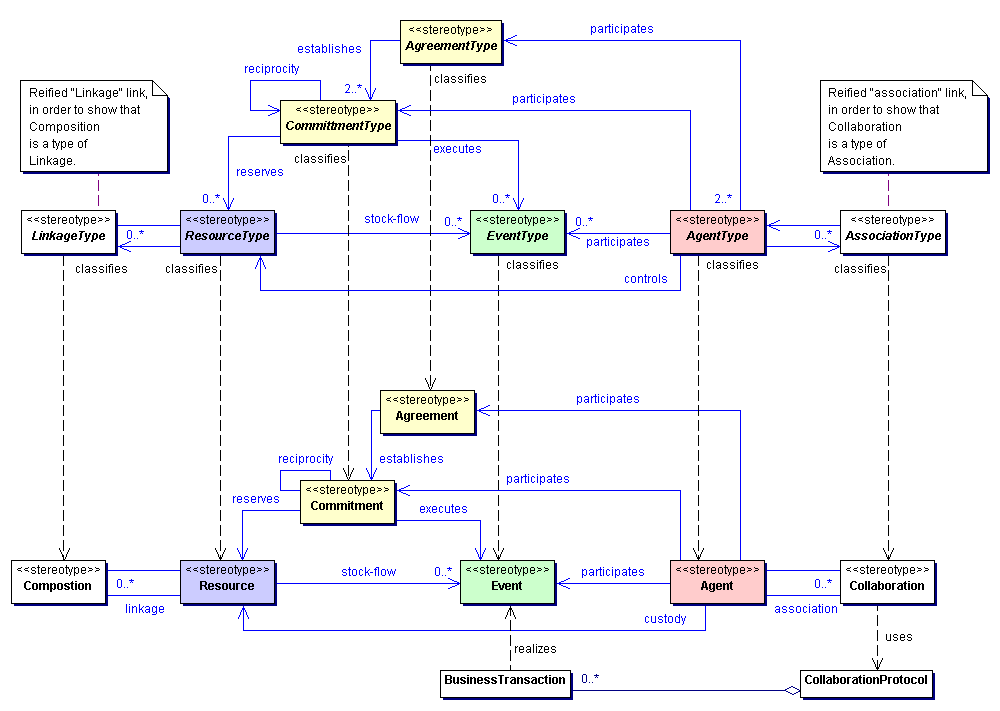
\includegraphics[width=90mm]{img/uvodni_obrazek.png}
	\caption{Příklad UML diagramu}
\end{figure}
	
\end{frame}

%%%%%%%%%%%%%%%%%%%%%%%%%%%%%%%%%%%%%%%%%%%%%%%%%%%%%%%%%%%%%%%%%%%%%%%%
%% Slide

\begin{frame}{Úvod}

\begin{block}{Wikipedia}
	\structure{UML}, Unified Modeling Language je v softwarovém inženýrství 
	grafický jazyk pro vizualizaci, specifikaci, navrhování a 
	dokumentaci programových systémů. 
\end{block}

\pause

\begin{itemize}
	\item<+-> Univerzální
	\item<+-> Standardizovaný
	\onslide<+->
	\begin{itemize}
		\item Object Management Group (OMG)
		\item UML 2.3 - květen 2010
	\end{itemize}
	\item<+-> Formální specifikace
	\item<+-> Jednoduché i složité aplikace
	\item<+-> Je rozšiřitelný
	\onslide<+->
	\begin{itemize}
		\item Stereotypes, OCL, Tagged Values
	\end{itemize}
\end{itemize}
	
\end{frame}

%%%%%%%%%%%%%%%%%%%%%%%%%%%%%%%%%%%%%%%%%%%%%%%%%%%%%%%%%%%%%%%%%%%%%%%%
%% Slide

\begin{frame}{Použití}

\onslide<+-> K čemu je UML?

\begin{itemize}[<+->]
	\item UML je nástroj, neudělá práci za nás
	
	\item Standardní způsob, jak se dorozumět s ostatními
	\begin{itemize}
		\item Je dobré znát aspoň základní diagramy
	\end{itemize}
	
	\item Návrh aplikace
	\begin{itemize}
		\item Zachycení myšlenek do vizuální podoby
	\end{itemize}

	\item Dokumentace
	\begin{itemize}
		\item Nelze v něm zachytit kompletní dokumentaci
	\end{itemize}
\end{itemize}

\onslide<+-> Jak ho používat?

\begin{itemize}[<+->]
	\item Standard neříká, který diagram ve které fázi použít
	\item Záleží na použité metodice nebo našem úsudku
	\begin{itemize}
		\item Pouze koncepty, třeba jen na papíře
		\item Důsledné modelování, detailní návrhy, nejrůznější nástroje
		\item Generování zdrojového kódu z UML diagramů
	\end{itemize}
	
	\item Použít tak, aby urychlilo a zjednodušilo práci
	\item Ne podřizovat způsob práce UML
\end{itemize}

\end{frame}

%%%%%%%%%%%%%%%%%%%%%%%%%%%%%%%%%%%%%%%%%%%%%%%%%%%%%%%%%%%%%%%%%%%%%%%%
%% Slide

\begin{frame}{Nevýhody}

\onslide<+-> UML je kritizováno

\begin{itemize}[<+->]
	\item Příliš objemný a formální standard
	\item Tak abstraktní, že se zdá, že se už vůbec nevztahuje k OOP
	\item Není úplně lehké se naučit
	\begin{itemize}
		\item Pro běžného člověka nemá smysl se učit detailně formální
		specifikaci
		\item Použití CASE nástroje na tvorbu diagramů, aniž známe 
		význam symbolů
	\end{itemize}	
	
	\item UML neodpovídá žádnému programovacímu jazyku
	\begin{itemize}
		\item Bylo by to zbytečné omezení
		\item Jiný způsob přemýšlení
		\item Není snadné generovat kód
		\item Občas něco problém vůbec implementovat
	\end{itemize}
	
	\item Výměna dat mezi jednotlivými nástroji
	\begin{itemize}
		\item Od verze 2.0 součástí standardu formát pro výměnu dat
		\item Není dostatečně detailní
		\item Některé nástroje možnost importu
		\item Ne vždy bez problémů
	\end{itemize}
\end{itemize}


\end{frame}

%%%%%%%%%%%%%%%%%%%%%%%%%%%%%%%%%%%%%%%%%%%%%%%%%%%%%%%%%%%%%%%%%%%%%%%%

